\section{Theorie}
\subsection{Das magnetische Moment der Elektronenhülle}
Das magnetische Moment der Elektronenhülle eines Atoms entsteht aus dem Zusammenspiel der magnetischen Momente der einzelnen Elektronen. Diese wiederum sind zurückzuführen auf die beiden bekannten Drehimpulse eines Elektrons:\\
Den Spin $\vec{s}$, mit
\begin{equation}
\abs{\vec{s}}=\sqrt{s(s+1)}\hbar\quad \text{mit } s=\frac{1}{2}\,,
\end{equation}
und den Bahndrehimpuls $l$
\begin{equation}
\abs{\vec{l}}=\sqrt{l(l+1)}\hbar\quad \text{mit } l=0,1,2....n-1\..
\end{equation}
Die daraus resultierenden magnetischen Momente sind:
\begin{equation}
\vec{\mu_l}=-\upmu_B\sqrt{l(l+1)}\vec{l_e}\,,
\end{equation}
wobei $\upmu_B$ das Bohrsche Magneton
\begin{equation}
\upmu_B=-\frac{1}{2}\text{e}_0\frac{\hbar}{\text{m}_0}\,,
\end{equation}
mit der Elementarladung $\text{e}_0$ und der Elektronenmasse $\text{m}_0$, ist und $\vec{l_e}$ ein Einheitsvektor in $\vec{l}$-Richtung ist und:
\begin{equation}
\vec{\mu_s}=-\text{g}_S\upmu_B\sqrt{s(s+1)}\vec{s_e}\,.
\end{equation}
Der hier auftretende Faktor $\text{g}_s\approx2$ ist dabei der Landé-Faktor des Elektrons, welcher für das anomale magnetische Moment des Spins verantwortlich ist und durch relativistische Effekte mit der Dirac-Gleichung erklärt werden kann.\\
Das magnetische Moment der kompletten Elektronenhülle entsteht dann durch die Wechselwirkung der Drehimpulse und magnetischen Momente aller Elektronen miteinander und jeweils für die einzelnen Elektronen. Da dieses System jedoch für die meisten Atome zu kompliziert wird, sind zwei mögliche Vereinfachungen möglich: für leichtere Atomkerne gilt die $L$-$S$-Kopplung, oder auch Russel-Saunders-Kopplung, während für schwere Kerne die $jj$-Kopplung genutzt wird.
\subsubsection{$L$-$S$-Kopplung}
Für leichtere Kerne dominiert die Wechselwirkung der Drehimpulse und magnetischen Momente der Elektronen untereinader, sodass sich jeweils ein Gesamtbahndrehimpuls
\begin{equation}
\vec{L}=\sum_i\vec{l}_i \quad\text{mit }\abs{\vec{L}}=\sqrt{L(L+1)}\hbar
\end{equation}
und ein Gesamtspin
\begin{equation}
\vec{S}=\sum_i\vec{s}_i \quad\text{mit }\abs{\vec{S}}=\sqrt{S(S+1)}\hbar
\end{equation}
bilden. Gesamtdrehimpuls und Gesamtspin für abgeschlossene Schalen sind dabei immer $0$, sodass nur unabgeschlossene betrachtet werden müssen. Aus historischen Gründen werden Gesamtbahndrehimpulsterme mit $L=0,1,2,3$ als S, P, D, F-Terme bezeichnet. Es können nur ganzzahlige Werte von $L$ auftreten. Als magnetisches Moment des Gesamtbahndrehimpuls ergibt sich
\begin{equation}
\abs{\vec{\mu_L}}=\upmu_B\sqrt{L(L+1)}
\end{equation}
und für den Gesamtspin
\begin{equation}
\abs{\vec{\mu_S}}=\text{g}_S\upmu_B\sqrt{S(S+1)}\,.
\end{equation}
Für hinreichend schwache externe Magnetfelder können sich dann Gesamtbahndrehimpuls und Gesamtspin zum Gesamtdrehimpuls der Elektronenhülle $\vec{J}$ zusammenschließen:
\begin{equation}
\vec{J}=\vec{L}+\vec{S} \quad\text{mit }\abs{\vec{J}}=\sqrt{J(J+1)}\hbar\,.
\end{equation}
Bei starken externen Magnetfelder hingegen tritt der Paschen-Back-Effekt auf und die $L$-$S$-Kopplung wird aufgehoben.
\subsubsection{$jj$-Kopplung}
Für schwere Kerne koppeln Spin und Bahndrehimpuls der einzelnen Elektronen zunächst aneinander, bevor sich ein Gesamtdrehimpuls aufstellen lässt. Es ergeben sich also die Gesamtdrehimpulse der einzelnen Elektronen $\vec{j}_i$
\begin{equation}
\vec{j}_i=\vec{l}_i+\vec{s}_i\,,
\end{equation}
aus welchen dann der Gesamtdrehimpuls der Elektronenhülle aufgestellt werden kann
\begin{equation}
\vec{J}=\sum_i\vec{j}_i\,.
\end{equation}
Der Übergang zwischen den Bereichen, in welchen die beiden Näherungen gültig sind, ist dabei fließend.\\
\newline
Das magnetische Moment der Elektronenhülle $\vec{\mu_J}$ ergibt sich aus den magnetischen Momenten $\vec{\mu_L}$ und $\vec{\mu_S}$
\begin{equation}
\vec{\mu_J}=\vec{\mu_L}+\vec{\mu_S} \quad \text{mit  } \abs{\vec{\mu_J}}=g_J\upmu_B\sqrt{(J(J+1)}\,,
\end{equation}
wobei $g_J$ ein Landé-Faktor ist
\begin{equation}
g_J=1+\frac{J(J+1)+S(S+1)-L(L+1)}{2J(J+1)}\,.
\end{equation}
Wegen der Richtungsquantelung hat der Winkel zwischen $\vec{\mu_J}$ und $\vec{B}$ nur Werte, bei denen für die Komponente in Feldrichtung gilt:
\begin{equation}
  \mu_{J_z}=-mg_J\upmu_B \,,
\end{equation}
wobei $m$ die magnetische Quantenzahl ist und ganzzahlige Werte zwischen $-J$ und $J$ annehmen kann.
\subsection{Aufspaltungen von Energieniveaus in externen Magnetfeldern}
Befindet sich ein Atom mit einem magnetischem Moment $\vec{\mu_J}$ in einem externen B-Feld, so existiert ein Energieterm $E_\text{mag}$ der Form
\begin{align}
E_\text{mag}&=-\vec{\mu_J}\cdot\vec{B}\\
&\text{bzw.}\nonumber\\
&=mg_J\upmu_B\,.
\end{align}
Es zeigt sich also, dass die Energieniveaus des Atoms in $2J+1$ äquidistante Unterniveaus aufspalten, wobei die Energiedifferenz der einzelnen Niveaus linear von der externen Feldstärke $\vec{B}$ abhängt.
Es folgt, dass durch die Aufspaltung auch neue Übergänge und somit neue Spektrallinien auftreten können. Auf die Regeln, die solche Übergänge befolgen müssen, soll im Folgenden weiter eingegangen werden.
\begin{figure}
  \centering
  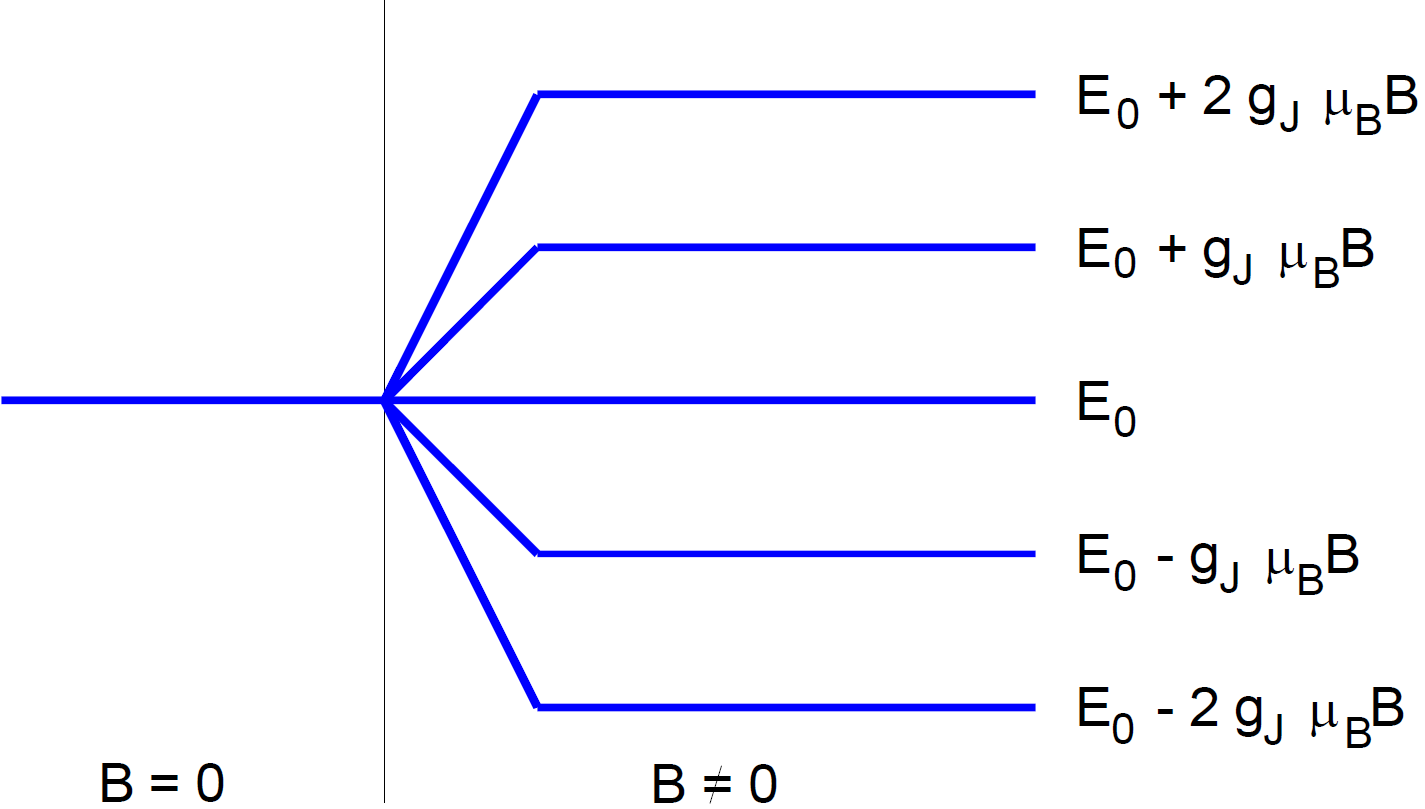
\includegraphics[width=0.7\textwidth]{Bilder/t1.png}
  \caption{Schematische Darstellung der Niveauaufspaltung eines Atoms mit $J=2$ in einem externen B-Feld.}
\end{figure}
\subsubsection{Übergangsregeln}
Durch Lösen der zeitabhängigen Schrödingergleichung für einen Übergang zwischen zwei Niveaus mit den Energien $E_m$ und $E_n$, was zur Emission eines Photons mit Frequenz
\begin{equation}
\nu_{mn}=\frac{E_m-E_n}{\text{h}}\,
\end{equation}
führen würde, lässt sich zeigen, dass die Übergangsregeln
\begin{align}
\upDelta l&=\pm1\newline\\
&\text{und}\nonumber\\
\upDelta m &=0,\pm1
\end{align}
erfüllt sein müssen. Ferner stellt sich heraus, dass diejenigen Übergänge, welche $\upDelta m=\pm 1$ haben, um die Feldachse zirkular polarisiert sind. Sie werden auch als $\upsigma^\pm$-Übergänge bezeichnet. Ein Übergang mit $\upDelta m=0$ wird hingegen als $\uppi$-Übergang bezeichnet und ist linear in Feldrichtung polarisiert.
\subsection{Der Zeeman-Effekt}
\subsubsection{Der normale Zeeman-Effekt}
Der aus historischen Gründen so benannte normale Zeeman-Effekt tritt in Atomen mit $S=0$ auf. Der verschwindende Gesamtspin bewirkt, dass die Energiedifferenz zwischen den einzelnen Zeemanniveaus stets gleich groß ist:
\begin{equation}
  \upDelta E=m\upmu_B B\,.
\end{equation}
Es entsteht also immer eine Aufspaltung in drei Liniengruppen mit gleichem $\upDelta m$.
\subsubsection{Der anomale Zeeman-Effekt}
Anders als beim normalen Zeeman-Effekt gilt hier $S\neq 0$, weswegen die Energiedifferenz hier mit variablen Landé-Faktoren durch
\begin{equation}
\upDelta E = \left(m_1 g(L_1,S_1,J_1)-m_2g(L_2,S_2,J_2)\right)\upmu_B B\,,
\label{eq:lande}
\end{equation}
gegeben ist.
\clearpage
